\documentclass[useAMS,usenatbib]{mn2e}
\usepackage[utf8]{inputenc}
\usepackage{graphicx}
\usepackage{amsmath}
\usepackage{amssymb}
%\usepackage[font={it},labelfont={bf}]{caption}
%\usepackage{units}
\usepackage{times}
\usepackage{color}
\usepackage[usenames,dvipsnames,svgnames,table]{xcolor}

\usepackage{fixltx2e} % fixes placing of image positions

\definecolor{customhdrcolor}{rgb}{0.0,0.0,0.0}
\definecolor{customcitecolor}{rgb}{0.0,0.5,0.75}
\definecolor{customlinkcolor}{rgb}{0.0,0.5,0.75}

\usepackage[colorlinks=true,linkcolor=customlinkcolor,urlcolor=customlinkcolor,citecolor=customcitecolor,pdftex]{hyperref}

\ifpdf\pdfinfo{/Title      (WSClean)
               /Author     (A. R. Offringa et al.)
               /Keywords   (instrumentation: interferometers;methods: observational;techniques: interferometric;radio continuum: general)
        }
\else\usepackage{graphics}\fi

\setlength{\pdfpageheight}{\paperheight}
\setlength{\pdfpagewidth}{\paperwidth}

%\newcommand{\editmark}[1]{#1}
%\newcommand{\editmark}[1]{{\color{red}{\textbf{#1}}}}

% To make Dutch ``tussenvoegsels'' work correctly in Latex such as ``de Bruyn'', we use this command
% It fixes ordering and uppercases.
% In text, it should be written with uppercase, as in ``De Bruyn''
\DeclareRobustCommand{\TUSSEN}[3]{#2}

\title[WSClean: a new imager]{WSClean: a new implementation of a fast, generic wide-field imager}

\author[A.~R.~Offringa et al.]{A.~R.~Offringa$^{1,2}$\thanks{E-mail:
\url{andre.offringa@anu.edu.au}}, B.~McKinley$^{1,2}$, N.~Hurley-Walker, 
F.~H.~Briggs, \newauthor
J.~Rhee, L.~Feng, D.~Kaplan, A.~R.~Neben, J.~D.~Hughes, MWA commissioning team\newauthor
and GLEAM members where appropriate \& MWA builders list
\\
$^{1}$RSAA, Australian National University, Mt Stromlo Observatory, via Cotter Road, Weston, ACT 2611, Australia \\
$^{2}$ARC Centre of Excellence for All-sky Astrophysics (CAASTRO) \\
}

\begin{document}

\date{Accepted TODO. Received TODO; in original form TODO}
\pagerange{\pageref{firstpage}--\pageref{lastpage}}
\pubyear{2014}

\label{firstpage}
\maketitle

\begin{abstract}
We present our new imager implementation, ``WSClean'', which we find to be an order of magnitude faster than existing implementations, as well as being capable of MWA full-sky imaging at full resolution.
TODO
\end{abstract}

\begin{keywords}
instrumentation: interferometers -- methods: observational -- techniques: interferometric -- radio continuum: general
\end{keywords}

\section{Introduction}

Observations from non-coplanar interferometric radio telescopes that image large fractions of the sky at once can not be imaged with simple imagers that are based on a two-dimensional Fast Fourier Transformation (FFT). Instead, the imaging algorithm needs to account for the ``w-term'' during inversion, which is the term that describes the deviation of the array from a perfect plane \citep{perley-noncoplanar-arrays}. This deviation is amplified for telescopes with wide field of view, making this especially an issue for low-frequency telescopes, that by nature are wide-field instruments.

There are several methods to deal with the w-term during imaging: facetting \citep{facetting-cornwell}, a three-dimensional Fourier transform \citep{perley-noncoplanar-arrays}, w-projection \citep{wprojection-cornwell}, w-stacking\footnote{TODO when/where was this first mentioned in literature?} \citep{widefield-imaging-ska-cornwell} and w-snapshots \citep{widefield-imaging-ska-cornwell}. The w-snapshots algorithm is a hybrid between snapshot imaging and one of the other w-term correcting techniques, most efficiently w-projection or w-stacking.

New generation of wide-field observatories are producing data sets that are orders of magnitude larger than before. Examples of such telescopes include the Murchison Widefield Array (MWA, \citealt{mwa}), the upgraded Jansky Very Large Array (JVLA) and the Low-Frequency Array (LOFAR, \citealt{lofar-2013}). At the MWA, some of the data is reduced with the w-projection algorithm implementation of the Common Astronomy Software Applications (CASA, \citealt{casa}). This is an attractive option because of its many features, high quality and free availability. However, at the MWA we have seen that a 2-min snapshot observation at low-elevation can take up to tens of hours with CASA's w-projection algorithm. Another option for reducing MWA data is the Real-Time System (RTS), which has been designed as an efficient calibrating and imaging pipeline specifically for MWA data \citep{rts-mwa}. It can use GPUs for improving efficiency, and uses a w-projection kernel during imaging to correct for the w-term. The kernel can be kept small, because the data is processed in snapshots that have been phase-centered to Zenith. The RTS can not perform deconvolution as of yet.

For the MWA it can be assumed that the ionosphere has the same effect on all tiles, because the maximum baseline length is relatively small (2.9~km) and smaller than the typical size of ionospheric structure (TODO cite). This is not the case for LOFAR, making it necessary to correct the direction-dependent ionospheric effects per station before gridding the data. The \texttt{awimager} has been written to perform these corrections, and uses a hybrid of a-projection, w-projection and w-stacking \citep{awimager-2013}.

Once the Square-Kilometre Array (SKA) begins its operation, the required computational power for wide-field imaging will become an even bigger challenge. In \citet{widefield-imaging-ska-cornwell}, it is shown that in theory the w-snapshots algorithm is an efficient approach for the SKA.

In this article, we present a new implementation of a generic wide-field imager that is significantly faster than CASA's w-projection implementation. To obtain the increase in speed, the implementation uses the w-stacking method for correcting the w-terms combined with snapshot imaging. We named the new imager ``WSClean'', as an abbreviation for ``W-Stacking Clean''. This work improves the field of wide-field imaging in the following ways:
\begin{itemize}
 \item The performance of a w-stacking implementation is compared to a w-projection implementation.
 \item The advantages of using the w-snapshots algorithm are analysed.
 \item Details are described of how to efficiently implement the w-stacking and w-snapshots algorithms.
 \item A new implementation is released, which we believe to be the fastest generic widefield imager available for many imaging scenarios.
\end{itemize}

The w-stacking algorithm is described in Sect.~\ref{sec:wstacking}. Details of implementing the w-stacking and w-snapshots algorithms are described in Sect.~\ref{sec:implementation}. Using various MWA observations, including observations with varying elevation, the performance will be analysed in Sect.~\ref{sec:analysis}.

\section{The w-stacking technique} \label{sec:wstacking}
In this section, we will describe the w-stacking algorithm from a mathematical point of view.

An interferometer samples the complex visibility function
\begin{align}\notag
V(u,v,w) = & \iint \frac{A(l,m) I(l,m)}{\sqrt{1-l^2-m^2}} \cdot \\ \label{eq:visibility-function}
& e^{-2\pi i \left(ul + vm + w(\sqrt{1-l^2-m^2}-1)\right)} dl dm,
\end{align}
where $u,v,w$ is a baseline coordinate in the coordinate system of the array, $A$ is the primary-beam function, $I$ is the sky function and $l,m$ are cosine sky coordinates. We will use $I'(l,m)$ to denote the sky function before primary-beam correction, $I'(l,m)=A(l,m)I(l,m)$. We will not discuss calibration, but assume $V$ has been calibrated before imaging. In the case of a polarized measurement, the symbols $V$, $A$ and $I$ are $2\times 2$ Jones matrices, but without loss of generality we will ignore polarization and treat inversion as a scalar problem. Imaging consists of inverting Eq.~\eqref{eq:visibility-function}, i.e., to find $I'$ from $V$.

For small field of views, the term $\sqrt{1-l^2-m^2}$ is approximately of unit size, making Eq.~\eqref{eq:visibility-function} approximate an ordinary 2-dimensional Fourier transform, which can be inverted with an inverse Fast Fourier Transform (FFT). A common rule is that this is valid when
\begin{equation}\label{eq:when-2d-is-valid}
\forall w,l,m: w\left(\sqrt{1-l^2-m^2}-1\right) \ll 1.
\end{equation}

To derive the w-stacking technique, Eq.~\eqref{eq:visibility-function} is rewritten to
\begin{align}\notag
V(u,v,w) = & \iint \frac{I'(l,m) e^{-2\pi i w(\sqrt{1-l^2-m^2}-1)}}{\sqrt{1-l^2-m^2}} \cdot \\ \notag
& e^{-2\pi i \left(ul + vm\right)} dl dm.
\end{align}
This is an ordinary two-dimensional Fourier transform going from $u,v$ space to $l,m$ space, and can be inverted to get:
% Intermediate step:
%\begin{align}\notag
%\frac{I'(l,m) e^{-2\pi i w(\sqrt{1-l^2-m^2}-1)}}{\sqrt{1-l^2-m^2}} = & \iint V(u,v,w) \cdot \\ \notag
%& e^{-2\pi i \left(ul + vm\right)} du dv,
%\end{align}
%which can be rewritten to
\begin{align}\notag
\frac{I'(l,m)}{\sqrt{1-l^2-m^2}} = & e^{2\pi i w(\sqrt{1-l^2-m^2}-1)} \iint V(u,v,w) \cdot \\ \notag
& e^{-2\pi i \left(ul + vm\right)} du dv.
\end{align}
Integrating both sides over $w_0$ to $w_e$, the minimum and maximum value of $w$, results in
\begin{align}\notag
\frac{I'(l,m)\left(w_e - w_0\right)}{\sqrt{1-l^2-m^2}} = \int\limits_{w_0}^{w_e} e^{2\pi i w(\sqrt{1-l^2-m^2}-1)} \cdot \\ \label{eq:wstacking}
\iint V(u,v,w)  e^{-2\pi i \left(ul + vm\right)} du dv dw.
\end{align}
The final step is to make the $u,v,w$ parameters discrete, so that the integration over $u$ and $v$ can become an inverse FFT and the integration over $w$ becomes a summation. This shows that the sky function can be reconstructed by i)~taking all samples that correspond to a specific value of $w$; ii)~grid those samples on a uniform grid; iii)~calculating the inverse FFT; iv)~apply the direction dependent phaseshift $e^{2\pi i w(\sqrt{1-l^2-m^2}-1)}$; v)~repeat this for all $w$-values and add the results together; vi)~apply the final scaling.

In practice, the final scaling will be different from $\left(w_e - w_0\right)/\sqrt{1-l^2-m^2}$ suggested by Eq.~\eqref{eq:wstacking}, because the individual $w$-layers will not be completely filled with samples. Therefore, the number of added samples and their weight have to be taken into account. Additionally, it might be required to divide out the effect of a possible convolution kernel, the primary beam and correct for other direction dependent effects. In XX, YY, LL or RR polarizations, a correlated baseline is the complex conjugate of the reversed baseline, and the relation $V(u,v,w)=\overline{V(-u,-v,-w)}$ holds. The right-hand side of Eq.\eqref{eq:wstacking} with only positive $w$-value samples then becomes the complex conjugate of the one with only negative $w$-values samples. In this case we can therefore calculate the image for $w<0$ from the image with $w>0$. That allows us to set $w_0$ to the minimum absolute $w$-value, which requires at least two times less layers. In any case, the input to the two-dimensional inverse FFT is not generally an Hermitian-symmetric function, and hence is always performed as a complex-to-complex transform. 

\subsection{Discretization of w} \label{sec:gridding-w}
While the discretization of $u$ and $v$ is similar to conventional imaging, the discretization of $w$ defines the number of w-layers that need to be processed. For this, one can use a rule similar to \eqref{eq:when-2d-is-valid}, and make sure that the phase difference for two subsequent discretized $w$-values, $w_A$ and $w_B$,  is less than one radian. This results in the constraint
\begin{equation} \label{eq:minimum-w-distance}
\left|\left(w_A - w_B\right) 2\pi (\sqrt{1-l^2-m^2}-1)\right| \ll 1.
\end{equation}
This suggest that a uniform discretization in $w$ is optimal TODO in contrast to some article? -- could be explained by having more samples at smaller $w$s. From Eq.~\eqref{eq:minimum-w-distance}, the required number of layers can be derived and is given by
\begin{equation} \label{eq:nwlayers-bound}
 N_\textrm{wlayers} \gg 2\pi \left(w_e - w_0\right) \max_{l,m} \left(1 - \sqrt{1-l^2-m^2}\right).
\end{equation}
Actual values for the right-hand side can differ a lot. The value of $w_e - w_0$ is influenced by the coplanarity of the array, the zenith angle and the wavelength, while the value of the $\max_{l,m}$ term is influenced by the angular size of the image. For the MWA, a typical value of $w_e - w_0$ is $\sim 10$ at zenith, but is already $\sim 400$ at a zenith angle of $30^{\circ}$. [TODO table of arrays with $w$ values at zenith/more angles/more freq?] For a typical full-field-of-view image of a MWA observation of $3072\times 3072$ pixels of $0.75''$ size, the $\max_{l,m}$ term is $0.68$. This implies that, in the case of the MWA, tens of $w$-layers are required at zenith and hundreds at lower elevations. The number of $w$-layers has a large effect on the performance of the $w$-stacking algorithm, and will be discussed further in section TODO.

\subsection{Time complexity of w-stacking}
It is useful to analyse the time complexity of w-stacking and compare it with w-projection, to understand which algorithm performs better in a given situation. We will use the following symbols: $N_\textrm{wlay}$ is the number of w-layers for w-stacking, $N_\textrm{pix}$ is the number of pixels in the image along each dimension, $N_\textrm{vis}$ is the number of visibilities and $N_\textrm{kern}$ is the size of the antialiasing kernel (see \S\ref{sec:gridding}), $N_\textrm{wkern}$ is the size of the w-kernel for w-projection, $w_e$ is the maximum $w$ value and $\alpha_\textrm{FOV}$ is the imaging field of view.

\begin{table}[h]
 \caption{Scaling of the computational cost for various imaging steps} \label{tbl:computational-cost-per-operation}
 \begin{tabular}{lll}
   \textbf{Operation} & \textbf{W-stacking} & \textbf{W-projection} \\
   \hline\hline
   Fourier transform(s) & $N_\textrm{wlay} N^2_\textrm{pix} \log N_\textrm{pix}$ & $N^2_\textrm{pix} \log N_\textrm{pix}$ \\
   W-term corrections   & $N_\textrm{wlay} N^2_\textrm{pix}$ & $N_\textrm{vis} N^2_\textrm{wkern}$ \\
   Gridding & $N_\textrm{vis}N^2_\textrm{kern}$ & $N_\textrm{vis} N_\textrm{kern}^2$ \\
   \hline\hline
 \end{tabular}
\end{table}

Table~\ref{tbl:computational-cost-per-operation} shows how the computational costs scale for the operations that dominate the imaging in the w-stacking and w-projection algorithms. For comparison, we can assume the gridding kernel adds a constant term and the terms $N_\textrm{wlay}$ and $N_\textrm{wkern}$ follow approximately $w_e \sin \alpha_\textrm{FOV}$. The time complexity for w-stacking is then given by
\begin{equation}
\textrm{TC}_\textrm{wstacking}=\mathcal{O}\left(N^2_\textrm{pix} \log N_\textrm{pix} w_e \sin \alpha_\textrm{FOV}+ N_\textrm{vis} \right),
\end{equation}
and for $w$-projection it is
\begin{equation}
\textrm{TC}_\textrm{wprojection}=\mathcal{O}\left(N^2_\textrm{pix} \log N_\textrm{pix} + N_\textrm{vis} w_e^2 \sin^2 \alpha_\textrm{FOV}\right).
\end{equation}
From these bounds it can be concluded that in the limiting behaviour, the $w$-stacking method will be faster when the gridding of the visibilities is the dominating cost of the algorithm. The $w$-projection algorithm will be faster when the inverse FFTs are dominating. In Sect.~\ref{sec:analysis} we will determine which method is faster in practice for different parameters.

\subsection{Full-sky imaging}
For low-frequency telescopes, it can be very useful to do full-sky imaging. In the case of MWA, the tile beam can have strong sidelobes at a distance of more than 90 degrees from the pointing centre. Imaging these sidelobes can be useful because there might be science (e.g. when searching for transients), or for self-calibration or full-sky deconvolution. The latter is for example useful when a strong source in a sidelobe affects the sensitivity in the pointing centre.

\subsection{W-snapshots}
TODO discuss projecting visibilities onto different tangent plane, imaging by small change to algorithm, output standard fits file by using CPIXij keyword \citet{wcs-in-fits}.
, and the w-terms can be kept small by phasing a snapshot to the orthogonal of the array's best-fitting plane

\section{The WSClean imager implementation} \label{sec:implementation}
We have implemented the $w$-stacking algorithm in the C++ language. Several steps are multi-threaded in this implementation: reading and writing, gridding from and to different $w$-layers, performing the Fast Fourier transforms and peak-finding and image subtraction during Cleaning. For the latter, intrinsics were used as well. This speeds up a minor Cleaning iterations, 

TODO discuss dealing with memory.

\subsection{Application of WSClean to the MWA}
The MWA correlator splits observations in data products of typically a few minutes
TODO

\section{Analysis} \label{sec:analysis}
TODO: Show image quality; show time-efficiency comparisons.

\subsection{Gridding} \label{sec:gridding}
During gridding of the visibilities in $uv$-space, it is useful to apply a gridding convolution kernel. A common kernel function is a windowed sinc function. A low-pass filter decreases the flux of sources outside the field of view, and thus helps to attenuate aliased ghost sources and sidelobes (see \citealt{post-correlation-filtering}) that arise because of the assumed periodicity during the inverse FFT. By supersampling, a convolution kernel also makes it possible to place samples more accurately at their $uv$ position, thereby lowering decorrelation.

The prolate spheroidal wave function (PSWF) is generally considered to be the optimal windowing function for gridding (TODO cite). CASA convolves samples with a PSWF of 7 pixels total width during gridding. When using a variable kernel size, a PSWF is quite complicated and computational expensive to calculate. WSClean currently uses a Kaiser-Bessel (KB) window function, which is easy and fast to compute, and its properties are similar to a PSWF.

\begin{figure}
\begin{center}
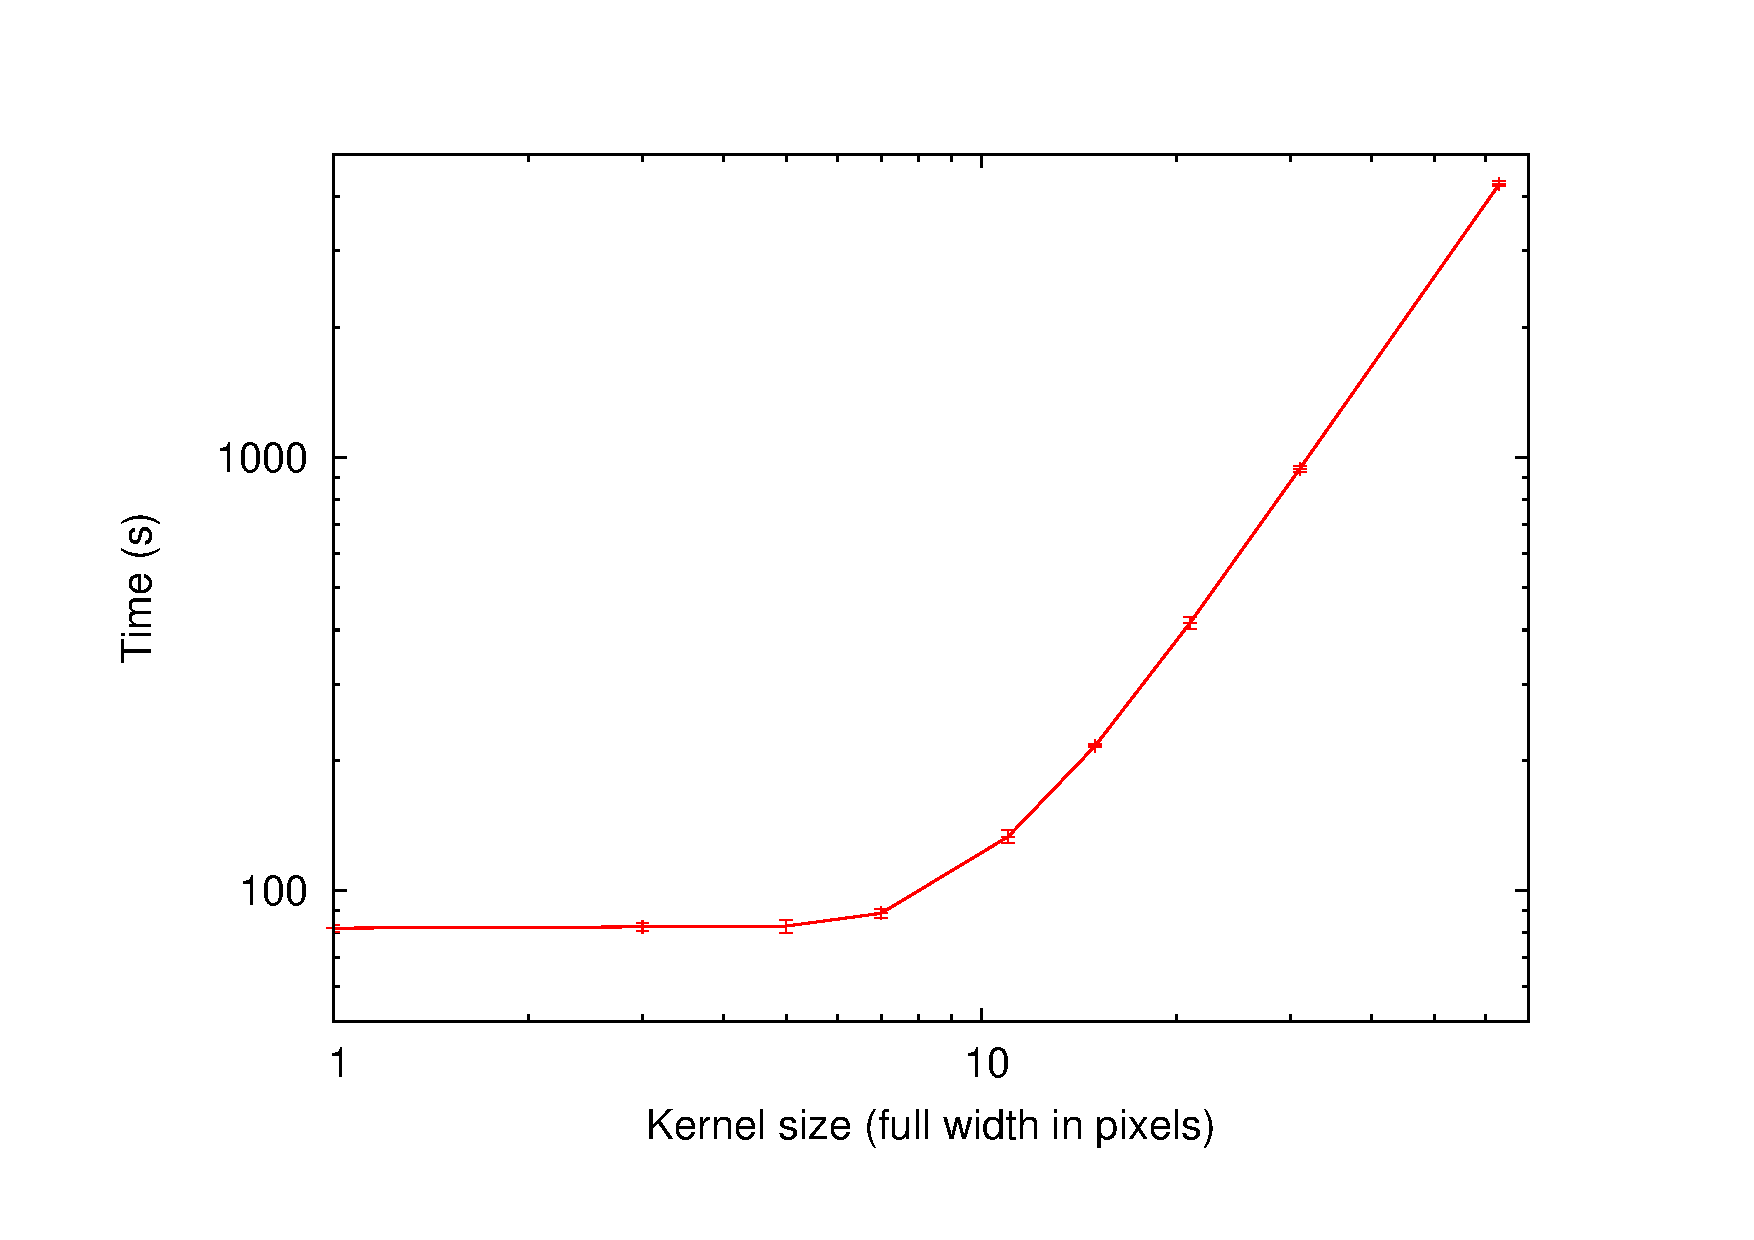
\includegraphics[width=8cm]{img/benchmark-kernelsize/kernel}
\caption{...}
\label{fig:timing-kernelsize}
\end{center}
\end{figure}

The type of window function has no effect on the gridding performance, but gridding has a quadratic time dependency on the size of the kernel. Fig.~\ref{fig:timing-kernelsize} shows that this quadratic dependency becomes apparent for kernel sizes $\ge 15$. Decreasing the kernel size to values below $7$ has little effect, because reading the samples takes more time than gridding with small kernels. We have not noticed much benefit of larger kernels except in rare cases where a bright source lies just outside the imaged field of view. Therefore, WSClean uses a default of 7 pixels for the gridding kernel. It can be increased when necessary.

\begin{table}
 \caption{Parameter values during benchmarks (unless the effect of the parameter was tested).}
 \begin{tabular}{lr}
   \textbf{Parameter} & \textbf{Value} \\
   Image size             & 3072 \\
   Number of visibilities & $10^9$
 \end{tabular}
\end{table}

\subsection{Cleaning a w-stacked image}
TODO describe how to do
TODO \citet{hogbom-clean}

It is tempting to use a very low number of $w$-layers, and define the major clean iteration threshold such that it will never clean any $w$-aliasing artefacts. However, predicting the visibilities from an image with a similar low number of $w$-layers will cause similar aliased errors, and thus will subtract incorrect fluxes from the visibilities. In the end, even though the sources causing the $w$-aliasing effects are removed, aliasing artefacts will still remain.

TODO: discuss low w-values means less-direction-invariant PSF.


\begin{figure}
\begin{center}
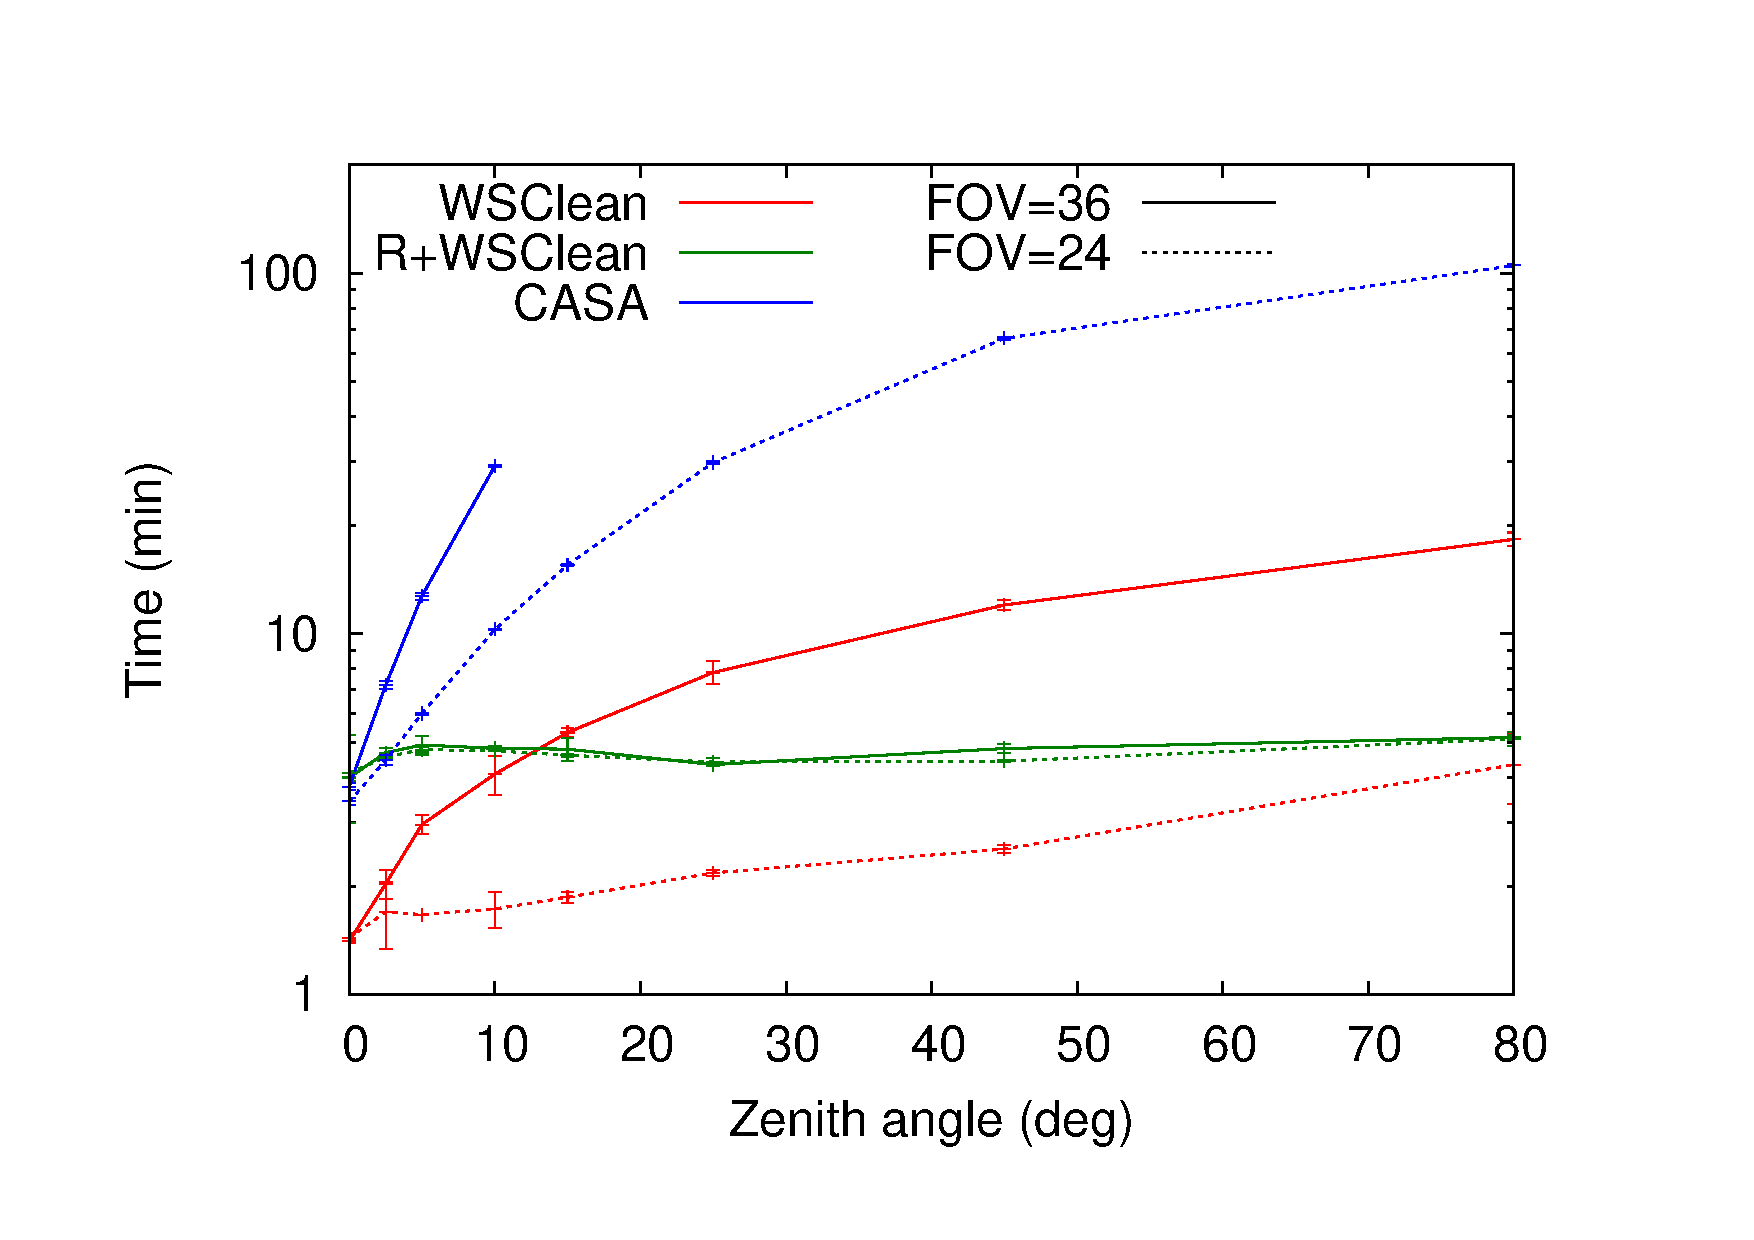
\includegraphics[width=8cm]{img/benchmark-zenith-angle/za}
\caption{...}
\label{fig:timing-zenith-angle}
\end{center}
\end{figure}

\begin{figure}
\begin{center}
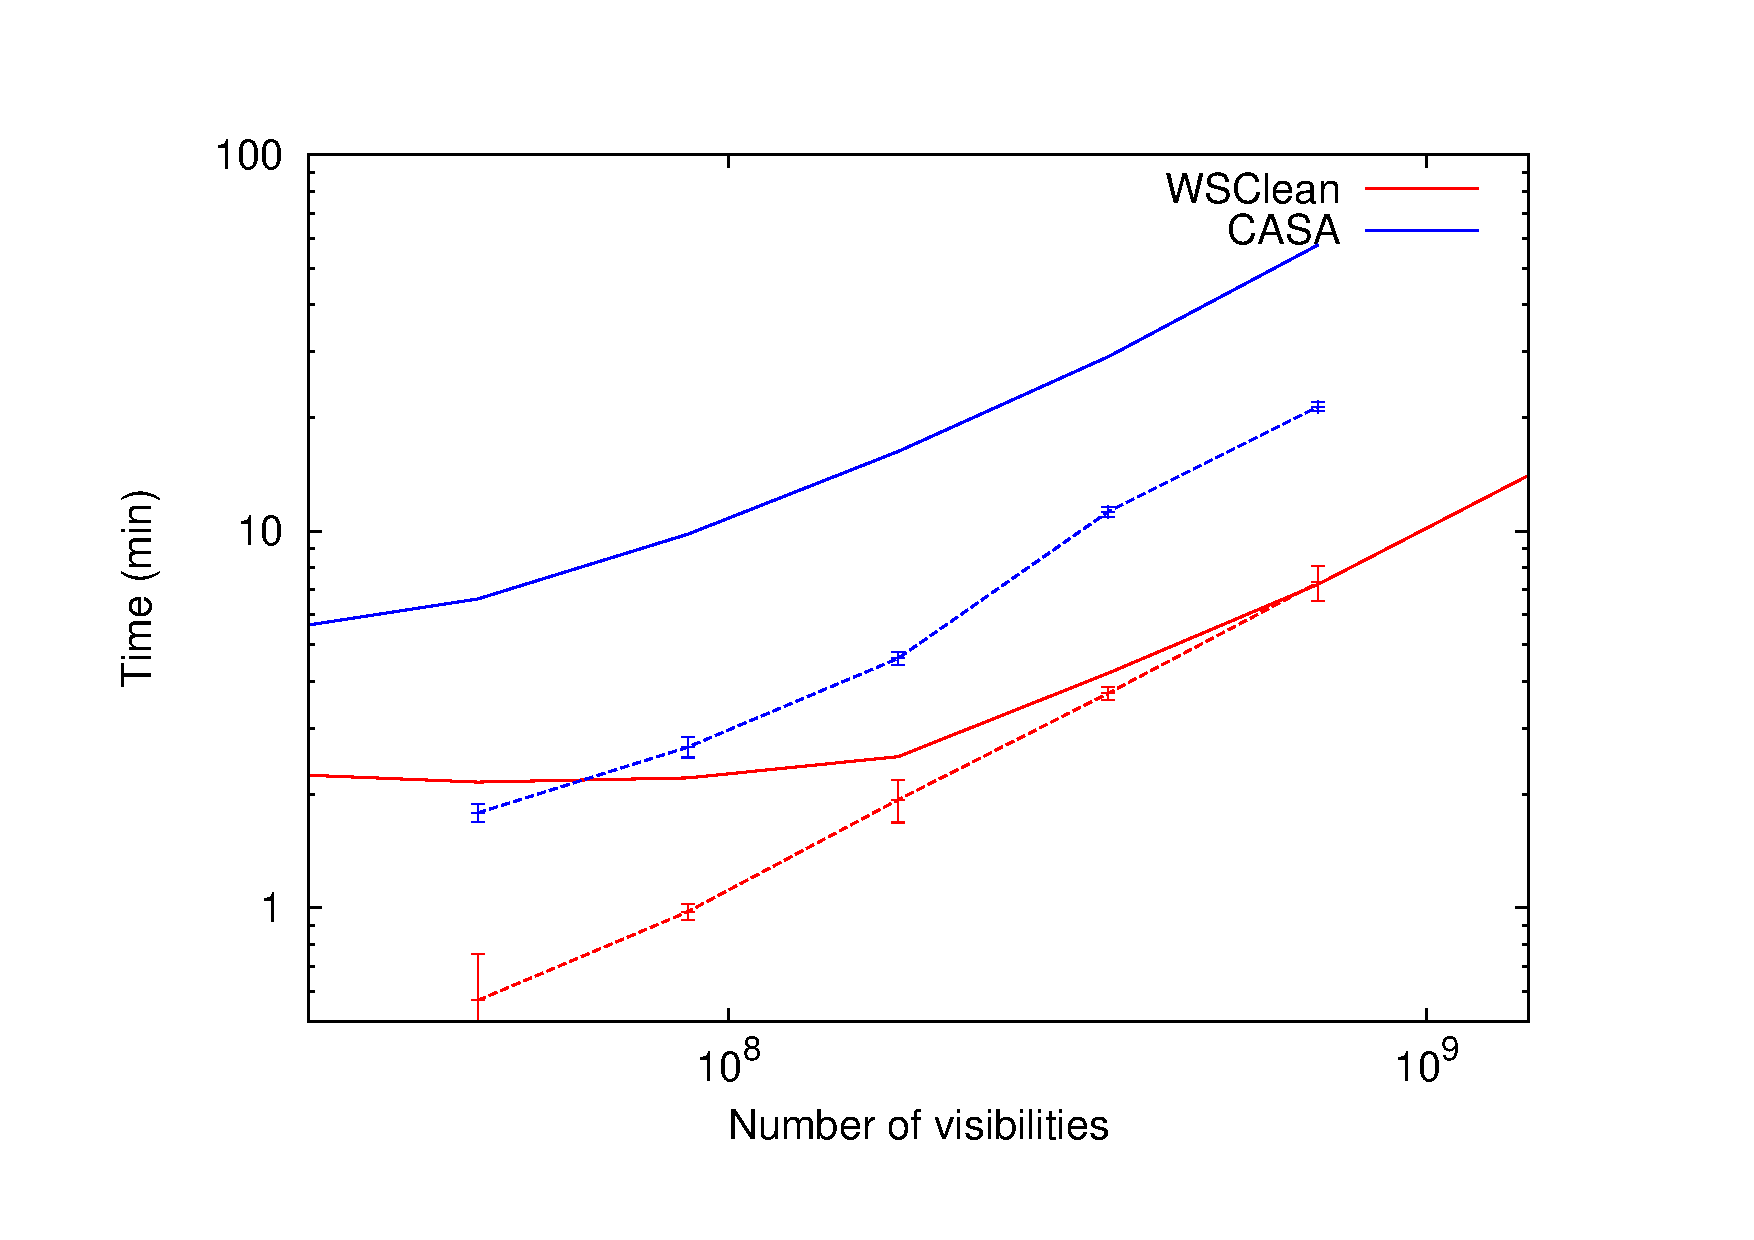
\includegraphics[width=8cm]{img/benchmark-nsamples/nsamples}
\caption{...}
\label{fig:timing-nsamples}
\end{center}
\end{figure}

\section{Discussion} \label{sec:discussion}
TODO: describe hybrid between w-stacking, w-projection and w-snapshots (if not yet discussed in Cornwell's papers)

TODO: A-projection makes the psf more invariant: therefore, truely ``joined'' deconvolution might be more accurate.

\section*{Acknowledgments}
...

% To make Dutch ``tussenvoegsels'' work correctly in Latex such as ``de Bruyn'', we use this command
% In bibliography, it should be written with lowercase, as in ``de Bruyn''
\DeclareRobustCommand{\TUSSEN}[3]{#3}

\bibliographystyle{mn2e}
\bibliography{references}

\label{lastpage}

\end{document}
